\documentclass[letterpaper,twocolumn,12pt]{article}
%\usepackage{verbatim}
\usepackage[]{graphicx}
\title{Classifying Protein Secondary Structures through Deep Network Learning}
\author{Stephanie deWet and Adam Vail}

\begin{document}
\maketitle

\section{Introduction}
\label{subsec:intro}
Predicting the underlying 3D structure of a protein from its amino acid sequence is a significant problem in structural molecular biology.
An important subproblem of this is to predict complex local structures, or secondary structures, from the amino acid sequence.  
The secondary structure problem has been attacked in a variety of ways, including with x-ray crystallography, biophysical models, and machine learning models.

Within in the field of machine learning, a variety of methods have been applied  over the past twenty years, with varying results. 
The majority of early work was done using standard neural networks with zero or one hidden layers resulting in the vast majority falling below 70\% accuracy.
The recent rise in popularity in deep networks (i.e. neural networks with multiple hidden layers) led us to investigate their accuracy in this problem space.

The common method of encoding amino acids uses large input vectors with an extremely sparse 1-ok-k representation.
Deep networks have the ability to reduce the dimensionality of large sparse feature spaces and are potentially well suited to simplifying the secondary structure problem.

\section{Related Works}
\label{subsec:relatedworks}
One of the earliest studies in this field was conducted by Qian and Sejnowski \cite{Qian} in 1988.
They experimented with using perceptrons and standard back-propagated single hidden layer neural networks.
They achieved results of 63.4\% accuracy which provides us with a reference point for our baselines.

Stolorz et al. combined perceptrons with bayesian methods to probabilistically inject domain knowledge into their model.
The combination of these two methods yielded an improvement over Qian with an accuracy of 64.4\%

Rost and Sander experimented with more complex network structures similar to deep networks.
They created an ensemble of complex networks consisting of two layers of standard single hidden layer neural networks, with the output of the first being the input of the second.
Within the ensemble, each network was trained using varying parameters in order to create separation between the models.
A majority vote was used to produce the final output which was modified in special cases using specific domain knowledge.
This method produced a significant increase in accuracy achieving 70.8\%.

\section{Method}
As alluded to in section \ref{subsec:intro}, our hypothesis is that a deep network has the ability to outperform a standard neural network on the protein secondary structure classification
problem.
Our objective is to find the optimal tuning of the deep network to yield the best predictive accuracy.

\subsection{Deep Networks Consisting of Stacked Autoencoders}
We choose a standard approach to creating a deep network by stacking varying numbers of autoencoders \cite{Hinton} which feed into a set of output units.
An autoencoder is a neural network with a single hidden layer that is trained using backpropagation to reproduce its inputs as outputs.
When there are less hidden units then inputs, the autoencoders enforces a more compact representation of the feature vector.
The process of creating a deep network consists of training a set stacked autoencoders using stochastic gradient descent where each successive autoencoder's inputs are the previous autoencoder's hidden layer.

\subsubsection{Input Encoding}
Our training data consists of a set of proteins, each of which is a variable length sequence of amino acids.
Each amino acid in the chain can take on one of twenty discrete values.
Therefore, there are two issues that must be overcome to use an amino acid sequence as input to a neural network: handling variable length inputs and modeling discrete values.

We model the discrete values by using a 1-of-k encoding.
Each amino acid is represented by twenty input nodes, one for each of its potential values.
Of the twenty input nodes, we set the input node corresponding to the amino acid's value to one and set all others to zero.
This was chosen because we did not want to impose an ordering on the values of the amino acid or to make certain values look artificially closer to each other.
Rost and Qian chose a similar encoding.

In order to handle variable length inputs and the fact that protein sequences tend to be quite long, we chose to use a sliding window over the sequence.
For every sliding window the goal is to classify the secondary structure of the amino acid at the center of the window.
The effect of changing the window size changes the impact of neighbors on the central amino acid's classification.
The challenge of using a sliding window is handling the amino acids that reside within half the window size of either end of the sequence.
We have chosen to model the ends of the sequence by setting each nonexistent (due to being off the end of the sequence) amino acid's twenty input nodes all to zero.
This method of using a sliding window was also used by Rost and Qian.

\subsubsection{Output Layer}
Our three classifications are the coarse secondary structures: alpha helix, beta sheet, or loop (known in some of the literature as coil).
We represent each of these possibilities with an output unit, where the highest value of the three output units is chosen in a winner-take-all fashion.
These outputs are attached to the hidden layer of the final autoencoder, and the resultant perceptrons are trained with back propagation using stochastic gradient descent.
We use a sigmoid function in all of the hidden and output units.

\subsection{Modifications to the Basic Algorithm}
\label{subsec:mods}
We have run some tests with each of the following modifications to the deep network.

\subsubsection{Decaying hidden layer size}
Because then input is a large sparse array, a more compact representation is desirable.
We use a decay factor to decrease the size of each stacked hidden layer, incrementally reducing the size of the feature space.
This is designed to find underlying structures in the data.

\subsubsection{Additional Connections to Output Units}
Due to the fact that the autoencoders find a compact representation of the data, we wanted to see whether we were losing valuable information in hidden layers.
We modified the output layer to connect to every input and hidden unit, so that the final layer has inputs from every layer of the deep network.
We then trained the final layer as a giant perceptron, and continued to use a winner-take-all final prediction.

\subsection{Baseline}
All previous work in section \ref{subsec:relatedworks} used domain knowledge in some form, we developed our own baseline model for comparison to our deep network.
The baseline is a standard neural network using a single hidden layer and trained with back propagation using stochastic gradient descent.

\subsubsection{Ensemble of Neural Networks}
The accuracy gained by Rost from the use of an ensemble inspired us to use an ensemble as well.
Unfortunately, due to the time complexity of convergence and limitations of physical compute resources, we were only able to develop this for the simpler baseline neural network.
A majority vote on the outputs of the individual neural networks was used to determine the final output of the ensemble.

\subsection{Verification}
All code for the baseline neural network and the deep network were verified by hand using small examples (no more than sequences of length greater than 5).
Specifically, we traced examples through a perceptron, standard single hidden layer neural network, autoencoder, and stacked autoencoders verifying their correctness.
In these tests, we found that small examples that were used for verification consistently required at least 1500 iterations over all the training data in order for the weights to converge.
Also, in the single-layer neural network test, we found that if the hidden layer size was too small, the autoencoder may be capable of re-creating the input, and each layer may converge, but the representation would be too compact for the full neural
Therefore, after many hours of debugging, we are confident the functionality of our learners are correct. 

\section{Empirical Evaluation}
As discussed in section \ref{subsec:intro}, the parameters we can optimize are sliding window size, hidden layer size, and number of hidden layers.
We constructed experiments to evaluate various settings of these parameters using both the deep network as well as the baseline neural network.
Due to the fact that the baseline consists of a single hidden layer, it converges more quickly that the deep network.
Therefore, we used results from the baseline to inform our choices of initial parameter settings when testing the deep network of autoencoders.
The basic algorithm modifications described in \ref{subsec:mods} were then evaluated using the best parameter settings from the other experiments.

\subsection{Dataset}
The datasets used by Rost and Qian were curated with significant domain knowledge therefore we chose to use a combination of these datasets.
Qian's dataset is currently hosted by the University of California - Irvine's (UCI) Machine Learning Repository \cite{uci}.
We used this data without any modification as it was already divided into a 91 protein training set and a test set of size 15 (resulting in 3500 windows of size 13).
The Rost data consists of 124 proteins.
Unfortunately, the exact data is not hosted for public use.
Therefore, we gathered the listed proteins using the Define Secondary Structure of Proteins (DSSP) database \cite{DSSP} \cite{DSSP2} to provide labels.
We followed the procedure in \cite{Rost} to group the eight secondary structure classes provided by DSSP into the three standard classes mentioned above.
We combined the Rost dataset with the Qian training data to create our training dataset, and used the UCI test set as our final test set.
Our parameter tuning experiments were tested using internal seven- or five- fold cross validation on the training data set.
(Earlier experiments used seven folds, but we switched to five-fold cross validation later due to time complexity.)
After we chose our parameter values, our final experiments were trained on the entire training set and then tested on the held-aside test set.
All plotted points in the following experiments are the average of the accuracies of each fold of the cross validation.

\subsection{Baseline Window Size}
Window size is important because it determines the number of neighbors that can influence an amino acid's classification.
Figure \ref{fig:baseline_window_size} shows that a window size of 13 or 17 was better than a smaller window.
This is to be expected, because a larger window uses results from sets a larger neighborhood around the central amino acid.
However, increasing the window size sharply increased the number of weights that needed to be trained.
As a compromise between accuraccy and performance, we chose to use a window size of 13 for all other experiments.

\begin{figure}[ht!]
\centering
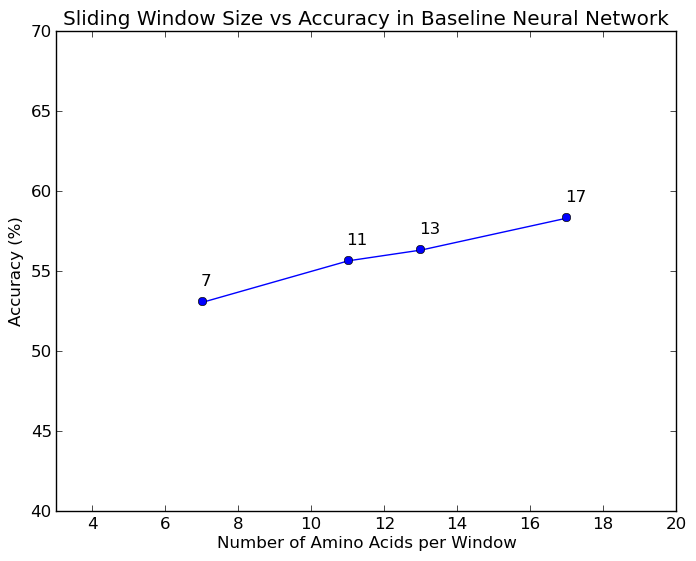
\includegraphics[width=65mm]{results/baseline/baseline_windowSize.png}
\caption{The effect of window size on accuracy, using a standard neural network. A window size of 13 was chosen for moving forward.}
\label{fig:baseline_window_size}
\end{figure}

\subsection{Baseline Hidden Layer Size}
Hidden layer size determines how much we compact the new representation of the inputs.
Figure \ref{fig:baseline_hidden_layer_size} shows that fewer units in the hidden layer represent the data better.
This shows that because the input data is extremely sparse, an entire window of amino acids can be encoded in very few hidden nodes.
Due to time complexity and physical computing resources, we couldn't test any networks with more than 200 hidden units, and could only test a handful of networks with more than 100 units.
Regardless, the data show that smaller numbers of hidden units per layer provide better prediction accuracy.
Based on these results, in subsequent experiments, we do not use more than 50 hidden units per layer.

\begin{figure}[ht!]
\centering
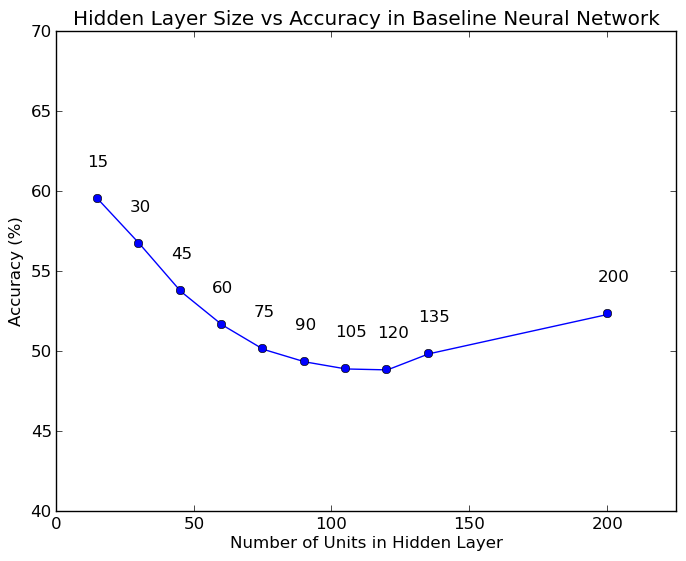
\includegraphics[width=65mm]{results/baseline/baseline_hiddenLayerSize.png}
\caption{The effect of hidden layer size, using a standard neural network.  Hidden layer sizes of less than 50 will be used moving forward.}
\label{fig:baseline_hidden_layer_size}
\end{figure}

\subsection{Deep Network}
In deep network tests, we used results from the baseline tests to set the window size to 13 and to choose a few good hidden layer sizes.
Figure \ref{fig:deep_num_hidden_layers} justifies our use of multiple hidden layer sizes.
It shows that a larger hidden layer is necessary when there are many hidden layers in the network.
This is consistent with the results of our single-layer neural network verification test, where a too-small hidden layer would strongly affect the network performance.  
In fact, we would expect any issues in early layers to be amplified in later layers, and to be even more obvious in networks with more layers.

The data show that the best accuracy occurs for a six hidden layer network.
Without domain knowledge, it's not clear what underlying physical structure each hidden layer represents, so we are unsure why some numbers of layers work better than others.
However, the network performance consistently increases  until it reaches six layers in size, after which point there is a large drop in accuracy.
We believe this is because six layers are capable of creating the most compact representation of the data the network can achieve, and additional layers simply introduce noise.

\begin{figure}[ht!]
\centering
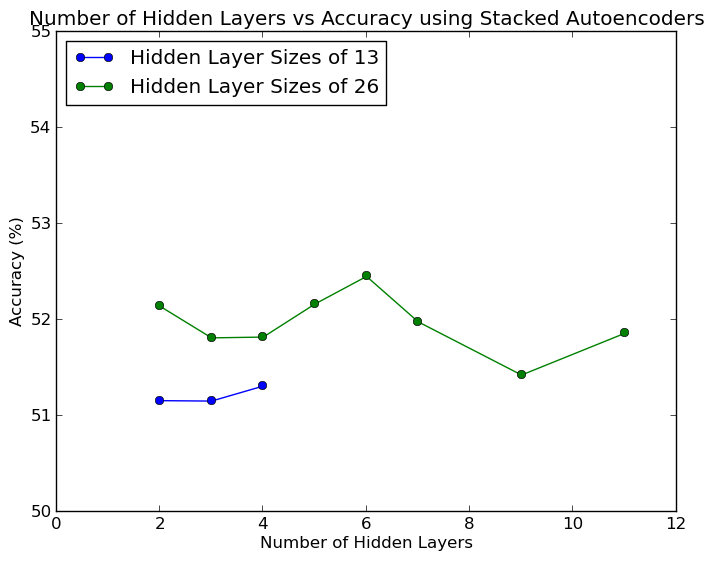
\includegraphics[width=65mm]{results/deep/deep_numLayers.png}
\caption{The effect of hidden layer size and number of hidden layers, using a deep network. The best average accuracy (52.5\%) was achieved using 6 hidden layers with 26 units per layer.}
\label{fig:deep_num_hidden_layers}
\end{figure}

\subsection{Decay}
In all of the deep network tests until this point, the sizes of all the hidden layers in a network were the same.
We modified our algorithm to use a decay factor, so that each hidden layer was some number of units smaller than the previous layer.
The first hidden for these tests has nearly fifty hidden units, so that the final layer sizes are not too small.

We found that these tests worked signifcantly worse than the standard deep networks.
Those tests achieved accuracies of approximately 52.5\%.
With three hidden layers, an initial hidden layer size of 45 and a decay factor of 25\%, we achieved an average accuracy of \textbf{50.37\%}.
With three hidden layers, an initial hidden layer size of 45 and a decay factor of 33\%, we achieved an average accuracy of \textbf{50.22\%}.

We hypothesize that this is because the network is being compacted too much at each step, to the point of losing information.


\section{Discussion}

% Insert and discuss ROC curves -- should I put ALPHA, BETA, LOOP on one plot?

As we mentioned in verication, if we used too few iterations for the network to converge, we saw a significant decrease in the performance of the network.

\section{Future Work}

\section{Conclusion}

\begin{thebibliography}{9}


\bibitem{Hinton}
G.E. Hinton and R. R. Salakhutdinov,
   `` Reducing the dimensionality of data with neural networks"
   in \emph{Science}, 2006.

\bibitem{DSSP}
Joosten RP, Te Beek TAH, Krieger E, Hekkelman ML, Hooft RWW, Schneider R, Sander C, Vriend G,
   `` A series of PDB related databases for everyday needs"
   in \emph{NAR}, 2010.

\bibitem{DSSP2}
Kabsch W, Sander C,
   `` Dictionary of protein secondary structure: pattern recognition of hydrogen-bonded and geometrical features"
   in \emph{Biopolymers}, 1983.

\bibitem{Qian}
Ning Qian and Terrence J. Sejnowski,
  `` Predicting the secondary structure of globular proteins using neural network models"
  in \emph{J. Mol. Bio.}, 1988.

\bibitem{Rost}
Burkhard Rost and Christ Sander,
  `` Prediction of protein secondary structures at bettter than 70\% accuracy"
  in \emph{J. Mol. Bio.}, 1993.

\bibitem{Stolorz}
Paul Stolorz, Alan Lapedes, and Yuan Xia,
   `` Predicting protein secondary structure using neural net and statistical methods"
   in \emph{J. Mol. Bio.}, 1992.

\bibitem{uci}
   C.L. Blake and C.J. Merz,
   `` UCI repository of machine learning databases"
   \textbf{http://archive.ics.uci.edu/ml/datasets/Molecular+Biology+(Protein+Secondary+Structure)}

\end{thebibliography}

\end{document}
